\documentclass[aspectratio=1610,onlymath]{beamer}
% \documentclass[aspectratio=1610,onlymath,handout]{beamer}

\input{macros-lecture}

\defineTitle{1}{Willkommen/Einleitung/Übersicht}{12. April 2021}

\begin{document}

\maketitle


\sectionSlide{Willkommen zur Vorlesung\\Theoretische Informatik und Logik}

% \begin{frame}\frametitle{}
%
% ~\hfill
% \includegraphics[height=6.5cm]{a1}
% \hfill~
%
% \end{frame}

\begin{frame}\frametitle{Raum, Zeit, URL}

\begin{itemize}
\item \emph{Vorlesungen:}\\
	In der Regel asynchron, Videos online\\
	Gelegentliche Konsultationstermine: Montag, DS2 (9:20--10:50)
% 	Donnerstag, DS4 (...), HSZ/0004\\
\item \emph{Keine Vorlesungen:}\\
	Ausfall: 13.5. (Himmelfahrt)\\
% 	Karfreitag: Fr 14.4.\\
% 	Dies academicus: Mi 17.5.\\
	Pfingstferien: Mo 24.5., Do 27.5.
\item \emph{Vorlesungswebseite}:\\[0.5ex]
	\url{\lectureurl}\\[0.5ex]
	(Folien, Übungsblätter, Termine, etc.)
\item \emph{Quellcode}:\\[0.5ex]
	\url{https://github.com/mkroetzsch/TheoLog}\\[0.5ex]
	(Fragen, Bug-Reports, Pull-Requests sind willkommen)
\item \emph{Matrix (Chat)}:\\[0.5ex]
	\url{https://matrix.tu-dresden.de/\#/room/\#theolog2021:tu-dresden.de}\\[0.5ex]
	(Support bei allen Fragen zur Vorlesung)
\end{itemize}

\end{frame}


\begin{frame}\frametitle{Übungen}
\begin{itemize}
\item \emph{Anmeldung} zu den Übungen über jExam
\item \emph{Übungsblätter} jeweils freitags für übernächste Woche
% \\
% 	(erstes Übungsblatt am 13. Oktober 2016)
\item \emph{Beginn der Übungen:} 19. April 2021
\item \emph{Übungsablauf}, vereinfacht, idealisiert:\\
	Aufgaben werden zu Hause bearbeitet so gut es geht;\\
	in der Übung helfen Gruppenleiter bei Fragen und Problemen und zeigen Beispiellösungen
% 	\pause\\[1ex]
% \item \emph{Motivation:}\\
% 	Die Klausur am Semesterende wird zwei Aufgaben enthalten, die zuvor in der Übung
% 	besprochen wurden
\end{itemize}

\end{frame}


\begin{frame}\frametitle{Prüfung und Prüfungsvorbereitung}
\begin{itemize}
\item schriftliche Prüfung (90min) am Ende des Sommersemesters, vermutlich online
\item prüfungsrelevant:\\
	kompletter Stoff aus Vorlesung \alert{und} Übung;\\
	Wiedergeben (Definieren), Anwenden (Rechnen) und Erklären (Beweisen)
\item Modulnote ergibt sich je nach Studiengang
\item zur zusätzlichen Vorbereitung gibt es \alert{mehrere Konsultationen} und \alert{eine Probeklausur}
\end{itemize}

\end{frame}


% \begin{frame}\frametitle{TheoLog Bestehen}
% Tipps:
% \begin{itemize}
% \item \emph{Von Hand Mitschreiben}\\
% 	{\footnotesize Man merkt sich Stoff deutlich besser, wenn man ihn für sich selbst handschriftlich
% 	zusammenfasst.\footnote{\tiny P.\ Mueller \& D.\ Oppenheimer. The Pen Is Mightier Than the Keyboard: Advantages of Longhand Over Laptop Note Taking. Psychological Science, 06/2014, 25:6}}
% \item \emph{Selber Rechnen}\\
% 	{\footnotesize Die Prüfung besteht im Lösen von Rechenaufgaben. Theorie allein hilft da nicht weiter.}
% \item \emph{Schnell sein}\\
% 	{\footnotesize Prüfungszeit ist meistens knapp. Es reicht nicht, Aufgaben "`im Prinzip"' lösen zu können. Man muss sie schnell lösen.}
% \item \emph{Ehrlich zu sich selbst sein}\\
% 	{\footnotesize Man sollte selbst wissen, ob man genug gelernt hat oder nicht.\footnote{\tiny Vgl.\ aber auch Wikipedia \href{https://de.wikipedia.org/wiki/Dunning-Kruger-Effekt}{[[Dunning-Kruger-Effekt]]}}}
% \end{itemize}
%
% \end{frame}


\sectionSlide{Motivation}

\begin{frame}\frametitle{Paris im August 1900}\label{frame_paris}

~\hfill
\includegraphics[height=6.5cm]{images/Paris-1900-Weltausstellung}
\hfill~

\end{frame}

\begin{frame}\frametitle{Der 2. Internationale Mathematikerkongress}\label{frame_hilbert}

\begin{minipage}{7cm}
\anybox{purple}{
"`Wer von uns würde nicht gern den Schleier lüften, unter dem die Zukunft verborgen liegt, um einen Blick zu werfen auf die bevorstehenden Fortschritte unsrer Wissenschaft und in die Geheimnisse ihrer Entwickelung während der künftigen Jahrhunderte!"'\\
\mbox{}\hfill-- David Hilbert, Paris, August 1900
}
\end{minipage}
\begin{minipage}{2.5cm}
~\hspace{8mm}
\includegraphics[width=2cm]{images/Hilbert}
\end{minipage}
\medskip\pause

Hilbert präsentiert eine Liste offener Fragen für die Mathematik des 20. Jahrhunderts:
\begin{itemize}
	\item 1. Problem: Kontinuumshypothese (und Auswahlaxiom)
	\item 2. Problem: Widerspruchsfreiheit der Arithmetik
	\item \ldots
\end{itemize}


\end{frame}

\begin{frame}\frametitle{Hilberts Programm}

Aber Hilberts wahres Ziel ist ein neues Verständnis der \ghost{Mathematik:}
\medskip

\anybox{purple}{
"`So unzugänglich diese Probleme uns erscheinen und so ratlos wir zur Zeit ihnen gegenüber stehen -- wir haben dennoch die sichere Ueberzeugung, daß ihre \alert{Lösung durch eine endliche Anzahl rein logischer Schlüsse} gelingen muß.

[\ldots]

Diese Ueberzeugung von der \alert{Lösbarkeit eines jeden mathematischen Problems} ist uns ein kräftiger Ansporn während der Arbeit; wir hören in uns den steten Zuruf: \alert{Da ist das Problem, suche die Lösung.} Du kannst sie durch reines Denken finden; denn in der Mathematik giebt es, kein Ignorabimus$^*$!"'
\\
\mbox{}\hfill-- David Hilbert, Paris, August 1900
}

$^*)$ lat. "`wir werden es niemals wissen"'
% \bigskip
%

\end{frame}

\begin{frame}\frametitle{Der Rest ist Geschichte \ldots}

\begin{itemize}
\item 1910--1913: Whitehead und Russel formalisieren in ihrer \alert{Principia Mathematica} logische Grundlagen der Mathematik\pause
\item 1918--1922: Hilbert spezifiziert sein Programm zur widerspruchsfreien Formalisierung der Mathematik\pause
\item 1928: Hilbert beschreibt das \alert{Entscheidungsproblem} der Prädikatenlogik\pause
\item 1929: Gödel beweist seinen \alert{Vollständigkeitssatz}: "`es gibt ein Kalkül, das alle Wahrheiten der Prädikatenlogik endlich beweisen kann"'\pause
\item 1936: Turing definiert ein universelles Rechenmodell: die \alert{Turingmaschine}\pause
\item 1951: Tarski publiziert ein Verfahren, mit dem alle wahren logischen Aussagen über reelle Zahlen, $+$ und $*$ automatisch durch Computer entschieden werden können
\end{itemize}

\end{frame}

\begin{frame}\frametitle{Der Rest ist Geschichte \ldots}

\begin{itemize}
\item 1976: Computerbeweis der Vier-Farben-Problems (Appel \& \ghost{Haken)}\pause
\item 1992: IBM's Supercomputer WHILE-S beweist die Fermatsche Vermutung\pause
\item ab 1995: erste Programmierumgebungen mit automatischer Verifikation\pause
\item 2001: IBM beweist die Goldbachsche Vermutung\pause
\item 2005: Google beweist die Riemannsche Vermutung\pause
\item 2007: "`American Mathematical Society"' benennt sich um in "`Association of Mathematical Programmers"'\pause
\item 2010: Zusammenbruch des Banksystems infolge der Veröffentlichung des Computerbeweises zur Entschlüsselung von Public-Key-Kryptographie\pause
\item 2013: Einstellung des Studiengangs Mathematik an der TU Dresden (Übertragung der Mathematiklehrer-Ausbildung an die Fakultät Informatik)
\end{itemize}

\end{frame}

\begin{frame}\frametitle{}

\pause
\begin{center}
{\huge\redalert{So ist es nicht gewesen.$^*$}}
\vspace{1cm}

\visible<3->{{\huge\alert{Warum nicht?}}}
\visible<4->{\vspace{5mm}

\begin{minipage}{7.5cm}
\begin{enumerate}[(A)]
\visible<4-7>{\item Historischer Zufall -- es kam einfach anders}
\visible<5-7>{\item Die Hardware ist noch nicht so weit}
\visible<6-7>{\item Die Software ist noch nicht so weit}
\visible<7-8>{\item Die beschriebene Entwicklung ist in unserem Universum unmöglich}
\end{enumerate}
\end{minipage}}
\end{center}
\vspace{1cm}

$^*)$ alle Ereignisse ab 1992 sind nie passiert

\end{frame}

\begin{frame}\frametitle{Informatik als Naturwissenschaft}

\anybox{strongyellow}{\vspace{-5mm}\begin{center}
Informatik erforscht, was Computer sind\\ und welche Probleme man mit ihnen lösen kann.\end{center}}\bigskip\pause

Computer = ein System das rechnet (CMOS-Schaltkreise, die Turingmaschine, DNA-Moleküle, ein quantenmechanisches System, das Universum, Minecraft, \ldots)
\bigskip

Ziel: universelle Erkenntnisse -- nicht nur über die Computertechnologie, die wir gerade nutzen, sondern über die Welt, in der wir leben  {\tiny wie Physik}
\bigskip

Methode: Spezifikation von einfachen Regeln, aus denen komplexe Systeme entstehen {\tiny anders als Physik, die mit dem System anfängt und dessen "`Regeln"' sucht}

\end{frame}

\begin{frame}\frametitle{Kernfragen der theoretischen Informatik}

\begin{itemize}
\item Was heißt "`berechnen"'?
\item Welche Probleme kann man auf reellen Computern lösen?
\item Was wäre, wenn wir mächtigere Computer hätten?
\item Was macht Rechenprobleme "`schwer"' oder "`einfach"'?
\item Sind alternative Rechenmodelle denkbar?
\item Welche (mathematischen/physikalischen/biologischen) Systeme können sonst noch rechnen?
\end{itemize}

Diese finden sich wieder in zahlreichen Teilgebieten (Berechenbarkeit, Automaten, Komplexität, Quantencomputing, logisches Schließen, künstliche Intelligenz, \ldots)

\end{frame}

\begin{frame}\frametitle{Übersicht "`TheoLog"'}

\alert{Teil 1: Berechenbarkeit}
\begin{itemize}
\item Turingmaschinen und andere Modelle
\item Entscheidbarkeit und unentscheidbare Probleme
\end{itemize}

\alert{Teil 2: Komplexität}
\begin{itemize}
\item Zeit und Raum
\item P, NP und PSpace
\end{itemize}

\alert{Teil 3: Prädikatenlogik}
\begin{itemize}
\item Syntax und Semantik
\item Modell-Checking (Anwendung: Datenbanken)
\item Logisches Schließen mit Resolution
\end{itemize}

\alert{Teil 4: Logik + Berechnung}
\begin{itemize}
\item Logik und formale Sprachen
\item Gödel
\item Weitere Themen \ldots
\end{itemize}

\end{frame}

% \overviewslide

\begin{frame}\frametitle{Literatur: Lehrbücher}

Der Vorlesungsstoff gehört zu fast jeder Informatikausbildung. Es gibt viele
Lehrmaterialien und eine weitgehend einheitliche \ghost{Notation.}
\bigskip

\begin{itemize}
\item Uwe Schöning: \emph{Theoretische Informatik -- kurz gefasst.} Spektrum Akademischer Verlag\\
{\footnotesize\textcolor{devilscss}{klassischer deutschsprachiger Text}}
%
\item Michael Sipser: \emph{Introduction to the Theory of Computation.}  Cengage Learning\\
{\footnotesize\textcolor{devilscss}{Standardtext zu Sprachen und Berechnungskomplexität}}
%
\item Christopher Moore, Stephan Meterns: \emph{The Nature of Computation.} Oxford University Press\\
{\footnotesize\textcolor{devilscss}{moderner Text zu Komplexität und Berechnung, weniger formell}}
\end{itemize}

Zu speziellen Themen der Logik werden wir bei Gelegenheit noch Literaturangaben machen.

\end{frame}

\begin{frame}\frametitle{Literatur: Mehr Bücher}

Teile des Stoffs der Vorlesung werden auch in vielen, zum Teil recht kurzweiligen
Büchern weniger formal behandelt, z.B.:
\bigskip

\begin{itemize}
\item Apostolos Doxiadis, Christos Papadimitriou:\\ \emph{Logicomix: An Epic Search for Truth.} Bloomsbury\\
{\footnotesize\textcolor{devilscss}{Graphic Novel, inspiriert von Russels Leben und der Geschichte der \ghost{Logik}}}
%
\item Scott Aaronson: \emph{Quantum Computing Since Democritus.} Cambridge\\
{\footnotesize\textcolor{devilscss}{eher informeller Text mit interessanten Denkanstößen}}
%
\item Douglas Hofstadter:\\ \emph{Gödel, Escher, Bach: An Eternal Golden Braid.} Basic Books\\
{\footnotesize\textcolor{devilscss}{der Klassiker}}
\end{itemize}

\end{frame}

\frame{\begin{center}\label{frame_turing_child}
\LARGE
Wiederholung: Turingmaschinen\bigskip

\includegraphics[height=5cm]{images/Turing-5.jpg}\\
{\tiny Alan Turing (5 Jahre alt)}
\end{center}}

\begin{frame}\frametitle{Turingmaschinen -- informell}

\emph{Schematische Darstellung:}\medskip

\narrowcentering{%
\begin{tikzpicture}[
	scale=0.50,
	decoration=penciline, decorate
]
% \path[use as bounding box] (-3.2,0) rectangle (3.5,-5); % add "draw" to see it
% \draw[help lines] (0,0) grid (5,5);
\pgfmathsetseed{5712}
%
\node (inlabel) [rectangle,draw=none,inner sep=1pt] at (3,0.5) {\alert{Eingabe-/Speicherband}};
\draw[decorate,line width=0.3mm] (-1,0) -- (10.5,0);
\draw[decorate,line width=0.3mm] (-1,-1) -- (10.5,-1);
\foreach \x in {0,...,10} {
	\draw[decorate,line width=0.3mm] (\x-1,0) -- (\x-1,-0.9);
	\node (s\x) [circle,draw=none,inner sep=1pt] at (\x-0.5,-0.5) {\ifthenelse{\x<5}{\ifthenelse{\x<3}{\Sterm{a}}{\Sterm{b}}}{\ifthenelse{\x=5 \OR \x=7 \OR \x=8}{\Snterm{C}}{\ifthenelse{\x=9}{\Sterm{b}}{\Snterm{D}}}}};
}
\draw[decorate,line width=0.3mm] (10,0) -- (10,-0.9);
\node (dots) [circle,draw=none,inner sep=1pt] at (11.1,-0.5) {$\cdots$};

% \draw[decorate,line width=0.3mm] (5.5,0) -- (6,0) -- (6,-0.9) -- (5.5,-0.9) ;
% \draw[decorate,line width=0.3mm] (6,0) -- (6,-0.9);

\draw[fill=none,decorate,line width=0.3mm]
	(2,-3) -- (6,-3) -- (6,-7) -- (2,-7) -- cycle;
\node (falabel) [circle,draw=none,inner sep=1pt,align=left] at (4,-5) {Endliche\\Steuerung};
\draw[fill=none,decorate,line width=0.4mm,darkblue,->]
	(4,-3) -- (4,-2) -- (6.5,-2) -> (6.5,-1);
\node (headlabel) [rectangle,draw=none,inner sep=1pt,align=left] at (9.5,-2.0) {\footnotesize\alert{Lese-/Schreibkopf}\\[-0.6ex]\footnotesize\alert{(beweglich)}};

\node[rectangle,align=center,draw,line width=0.3mm,decorate, minimum width=8mm, minimum height=8mm] (state) at (8, -6) {$q$};
\draw[fill=none,decorate,line width=0.4mm,darkblue,->]
	(6,-6) -> (state.180);
\node (qlabel) [rectangle,draw=none,inner sep=1pt] at (11.5,-6) {\footnotesize\alert{Zustandsvariable}};

% \node[cloud, cloud puffs=15.7, cloud ignores aspect, minimum width=4cm, minimum height=1cm, align=center, draw,line width=0.3mm] (memory) at (11, -1) {\alert{zusätzlicher}\\\alert{Speicher}};
%
% \draw[fill=none,decorate,line width=0.3mm] (9,0) -- (14,0);
% \draw[fill=none,decorate,line width=0.3mm] (9,-1) -- (14,-1);
% \draw[fill=none,decorate,line width=0.3mm] (9,0) -- (9,-1);
% \foreach \y in {10,...,14} {
% 	\draw[fill=none,decorate,line width=0.3mm] (\y,0) -- (\y,-0.9);
% 	\node (k\y) [circle,draw=none,inner sep=1pt] at (\y-0.5,-0.5) {\ifthenelse{\y<12}{\Snterm{A}}{\Snterm{B}}};
% }
% \draw[fill=none,decorate,line width=0.4mm,darkblue,->]
% 	(6,-3.5) -- (7.5,-3.5) -- (7.5,-0.5) -> (9,-0.5);
% \node (stacklabel) [circle,draw=none,inner sep=1pt] at (11.5,-1.5) {\alert{Warteschlange}};
\end{tikzpicture}}
\bigskip\pause

\emph{Übergangsfunktion:}
\begin{itemize}
\item \alert{Eingabe:} aktueller Zustand, gelesenes Zeichen
\item \alert{Ausgabe:} neuer Zustand, geschriebenes Zeichen, Änderung Lese-/Schreibadresse (${}\hat{=}{}$ Bewegung Lese-/Schreibkopf)
\end{itemize}

\end{frame}

\begin{frame}\frametitle{Definition DTM}

\defbox{Eine \redalert{deterministische Turingmaschine} (DTM) ist ein Tupel
$\Smach{M}=\tuple{Q,\Sigma,\Gamma,\delta,q_0,F}$ mit
den folgenden Bestandteilen:
\begin{itemize}
\item $Q$: endliche Menge von \redalert{Zuständen}
\item $\Sigma$: \redalert{Eingabealphabet}
\item $\Gamma$: \redalert{Arbeitsalphabet} mit $\Gamma\supseteq\Sigma\cup\{\blank\}$
\item $\delta$: \redalert{Übergangsfunktion}, eine partielle Funktion\\[1ex]
\narrowcentering{$Q\times\Gamma \to Q\times\Gamma\times\{L,R,N\}$}
\item $q_0$: \redalert{Startzustand} $q_0\in Q$
\item $F$: Menge von akzeptierenden \redalert{Endzuständen} $F\subseteq Q$
\end{itemize}
}

\alert{Dabei bedeutet $\delta(q,a)=\tuple{p,b,D}$:}\\
\hspace{5mm}"`Liest die TM in Zustand $q$ unter dem Lese-/Schreibkopf ein $a$,\\
\hspace{5.8mm}dann wechselt sie zu Zustand $p$, überschreibt das $a$ mit $b$\\
\hspace{5.8mm}und verschiebt den Lese-/Schreibkopf gemäß $D\in\{L,R,N\}$\\
\hspace{5.8mm}(nach links, nach rechts, gar nicht)."'

\end{frame}

\begin{frame}\frametitle{Definition NTM}

\defbox{Eine \redalert{nichtdeterministische Turingmaschine} (NTM) ist ein Tupel
$\Smach{M}=\tuple{Q,\Sigma,\Gamma,\delta,q_0,F}$ mit
den folgenden Bestandteilen:
\begin{itemize}
\item $Q$: endliche Menge von \redalert{Zuständen}
\item $\Sigma$: \redalert{Eingabealphabet}
\item $\Gamma$: \redalert{Arbeitsalphabet} mit $\Gamma\supseteq\Sigma\cup\{\blank\}$
\item $\delta$: \redalert{Übergangsfunktion}, eine totale Funktion\\[1ex]
\narrowcentering{$Q\times\Gamma \to 2^{Q\times\Gamma\times\{L,R,N\}}$}\\
wobei $2^{Q\times\Gamma\times\{L,R,N\}}$ die Potenzmenge von $Q\times\Gamma\times\{L,R,N\}$ ist
\item $q_0$: \redalert{Startzustand} $q_0\in Q$
\item $F$: Menge von akzeptierenden \redalert{Endzuständen} $F\subseteq Q$
\end{itemize}
}

\alert{Dabei bedeutet $\tuple{p,b,D}\in\delta(q,a)$:}\\
\hspace{5mm}"`Liest die TM in Zustand $q$ unter dem Lese-/Schreibkopf ein $a$,\\
\hspace{5.8mm}dann \alert{kann} sie zu Zustand $p$ wechseln, $a$ mit $b$ überschreiben\\
\hspace{5.8mm}und den Lese-/Schreibkopf gemäß $D\in\{L,R,N\}$ verschieben."'

\end{frame}

\begin{frame}\frametitle{Beispiel}

\emph{Wir können TMs in Diagrammen darstellen:}\medskip

Ein Pfeil $s_1\mapsto s_2,D$ von $q_1$ nach $q_2$ bedeutet\\
$\delta(q_1,s_1)=\tuple{q_2,s_2,D}$ (DTM) bzw. $\tuple{q_2,s_2,D}\in\delta(q_1,s_1)$ (NTM)
\bigskip

\emph{Beispiel:}\medskip

\begin{center}
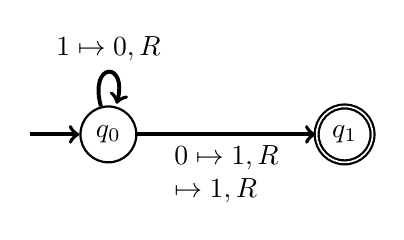
\begin{tikzpicture}[baseline={(q1.base)}]
% \draw[help lines] (0,0) grid (7,2);
\node (q1) [circle,draw=black,thick] at (0,0) {$q_0$};
\node (q2) [circle,double,draw=black,thick] at (3,0) {$q_1$};
%
\path[->,line width=0.5mm](-1,0) edge (q1);
\path[->,line width=0.5mm](q1) edge node[below,align=left] {$\Sterm{0}\mapsto\Sterm{1},R$\\$\blank\mapsto\Sterm{1},R$} (q2);
\path[->,line width=0.5mm](q1) edge[loop above] node[above] {$\Sterm{1}\mapsto\Sterm{0},R$} (q1);
\end{tikzpicture}
\end{center}

NTM oder DTM? Was tut diese Turingmaschine?

\end{frame}

\begin{frame}\frametitle{TM: Beispiel Abarbeitung}

TMs gehen schrittweise von einer Konfiguration in die nächste über:

\begin{center}
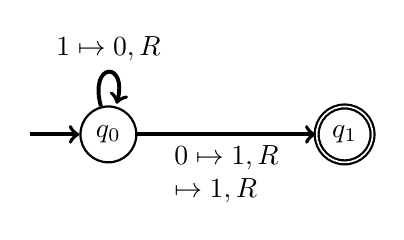
\begin{tikzpicture}[baseline={(q1.base)}]
% \draw[help lines] (0,0) grid (7,2);
\node (q1) [circle,draw=black,thick] at (0,0) {$q_0$};
\node (q2) [circle,double,draw=black,thick] at (3,0) {$q_1$};
%
\path[->,line width=0.5mm](-1,0) edge (q1);
\path[->,line width=0.5mm](q1) edge node[below,align=left] {$\Sterm{0}\mapsto\Sterm{1},R$\\$\blank\mapsto\Sterm{1},R$} (q2);
\path[->,line width=0.5mm](q1) edge[loop above] node[above] {$\Sterm{1}\mapsto\Sterm{0},R$} (q1);
\end{tikzpicture}
\end{center}

Eingabe: $\Sterm{1101}$\bigskip\pause

$q_0\Sterm{1101}\pause\vdash \Sterm{0}q_0\Sterm{101}\pause\vdash \Sterm{00}q_0\Sterm{01}\pause\vdash \Sterm{001}q_1\Sterm{1}$
\bigskip\pause

Ausgabe: $\Sterm{0011}$

\end{frame}

\begin{frame}\frametitle{Wiederholung Grundbegriffe}

\redalert{Konfiguration:} der "`Gesamtzustand"' einer TM, bestehend aus Zustand, Bandinhalt und Position des Lese-/Schreibkopfs;\\[1ex]
geschrieben als Wort (Bandinhalt), in dem der Zustand vor der Position des Kopfes eingefügt ist
\bigskip

\redalert{Übergangsrelation:} Beziehung zwischen zwei Konfigurationen, wenn die TM von der ersten in die zweite übergehen kann (deterministisch oder nichtdeterministisch); geschrieben als $\vdash$
\bigskip

\redalert{Lauf:} mögliche Abfolge von Konfigurationen einer TM, beginnend mit der Startkonfiguration; kann endlich oder unendlich sein
\bigskip

\redalert{Halten:} Ende der Abarbeitung, wenn die TM in einer Konfiguration keinen Übergang mehr zur Verfügung hat

\end{frame}

\begin{frame}\frametitle{Was ist das Ergebnis einer TM-Berechnung?}

Es gibt zwei wesentliche Arten DTMs zu benutzen:

\begin{enumerate}[(1)]
\item \alert{Transducer:} Ausgabe der TM ist der Inhalt des Bandes, wenn sie hält, oder undefiniert, wenn sie nicht hält (partielle Funktion); Endzustände spielen keine Rolle und können weggelassen werden
\item \alert{Entscheider:} Ausgabe der TM hat nur zwei Werte: die TM "`akzeptiert"', wenn sie in einem Endzustand hält und sie "`verwirft"' wenn sie in einem Nichtendzustand oder gar nicht hält;
Bandinhalt beim Halten spielt keine Rolle und kann ignoriert werden
\end{enumerate}

Wir werden NTMs nur als Entscheider verwenden: in diesem Fall reicht es, wenn mindestens ein möglicher Lauf akzeptiert.

\end{frame}

\begin{frame}\frametitle{NTM, DTM und die Church-Turing-These}

Wir wissen: {\tiny(aus "`Formale Systeme"', Winter 2020/2021, 19. Vorlesung)}

\theobox{\emph{Satz:} Jede NTM kann durch eine DTM simuliert werden. Insbesondere akzeptieren deterministische und nichtdeterministische Turingmaschinen dieselben Sprachen.}
\pause

Allgemeiner gilt: kein bekanntes Berechnungsmodell kann mehr berechnen als TMs

\anybox{purple}{\emph{Church-Turing-These:} Jede (partielle) Funktion, die intuitiv als berechenbar angesehen werden kann, ist auch mit einer Turingmaschine berechenbar.}

\begin{itemize}
\item \emph{Lesart 1:} Vorschlag einer mathematischen Definition der intuitiven Idee von Berechenbarkeit
\item \emph{Lesart 2:} "`Naturgesetz"' über die Möglichkeiten und Grenzen des Rechnens an \ghost{sich}
\end{itemize}

\end{frame}

\begin{frame}\frametitle{Zusammenfassung und Ausblick}

Die Theorie der Informatik untersucht Systeme im Hinblick auf ihre Fähigkeit zur Informationsverarbeitung (Berechnung)
\bigskip

Grundbegriffe: Turingmaschine (det./nichtdet.), Konfiguration, Lauf, Akzeptanz
\bigskip

Church-Turing-These: "`Alle Computer sind gleich"'
\bigskip

\anybox{yellow}{
Was erwartet uns als Nächstes?
\begin{itemize}
\item Probleme
\item Paradoxien
\item Phänomenal große Zahlen
\end{itemize}
}

\end{frame}

\begin{frame}[t]\frametitle{Bildrechte}

Folie \ref{frame_paris}: Fotografie von 1900, gemeinfrei\\
Folie \ref{frame_hilbert}: Fotografie von 1912, gemeinfrei\\
Folie \ref{frame_turing_child}: Fotografie von 1917, gemeinfrei\\

\end{frame}


\end{document}
